% Find documentation here:
% - https://ctan.org/pkg/tudscr?lang=en
% - https://github.com/tud-cd/tudscr/blob/main/source/doc/examples/poster.tex

\RequirePackage{fix-cm}
\documentclass[%
  english,%
  paper=A1,%
  fontsize=22pt,%
  cdfoot=5ex,%
  ddcfoot,%
  %shift text format field left and right
  BCOR=-20mm,
]{tudscrposter}

\usepackage[T1]{fontenc}
\usepackage{babel}
\usepackage{import}
\usepackage{blindtext}
\usepackage{multicol}
\usepackage{tabularx}
\usepackage{qrcode}
\usepackage{graphicx}
\usepackage{tikz}
\usetikzlibrary{backgrounds}
\usepackage{svg}
\usepackage{pdfpages}
\usepackage{wrapfig}
\usepackage{xcolor}
\usepackage[export]{adjustbox}
\usepackage{tcolorbox} % farbige Boxen


\definecolor{messagespace}{HTML}{e6c6d9}
\definecolor{messageselection}{HTML}{9bcff2}
\definecolor{encoding}{HTML}{73c2aa}
\definecolor{tagextraction}{HTML}{f0c985}
\definecolor{tagcomparison}{HTML}{f6ee91}


% --- Math Packages ---
\usepackage{amsmath}        % Advanced math environments
\usepackage{amssymb}        % Extra math symbols
\usepackage{mathtools}      % Further math tools, loads amsmath
\usepackage{commath}        % For common math commands like \dif
\usepackage{amsthm}         % For theorem and proof environments


\usepackage[acronym]{glossaries} % 
% \newacronym{tsn}{TSN}{Time-Sensitive Networking}
\newacronym{fifo}{FIFO}{First-In-First-Out}
\newacronym{qos}{QoS}{Quality-of-Service}
\newacronym{tas}{TAS}{Time-aware Shaper}
\newacronym{spq}{SPQ}{Strict Priority Queuing}
\newacronym{af}{AF}{Application Function}
\newacronym{upf}{UPF}{User Plane Function}
\newacronym{tt}{TT}{TSN Translator}
\newacronym{dstt}{DS-TT}{Device-Side TSN Translator}
\newacronym{nwtt}{NW-TT}{Network-Side TSN Translator}
\newacronym{gui}{GUI}{Graphical User Interface}
\newacronym{sdr}{SDR}{Software-defined Radio}
\newacronym{ue}{UE}{User Equipment}
\newacronym{cots}{COTS}{Commercial-off-the-Shelf}
\newacronym{ptp}{PTP}{Precision Time Protocol}
\newacronym{ran}{RAN}{Radio Access Network}
\newacronym{TI}{TI}{Tactile Internet} % Assuming you have this file
% \newcommand{\rarrow}{$\rightarrow$ }

%Mathematische Notation der gängigen Mengen
\newcommand{\RR}{\mathbb{R}} %reelle Zahlen
\newcommand{\CC}{\mathbb{C}} %komplexe Zahlen
\newcommand{\QQ}{\mathbb{Q}}
\newcommand{\NN}{\mathbb{N}}
\newcommand{\ZZ}{\mathbb{Z}}
\newcommand{\Prob}{\mathbb{P}} % Wahrscheinlichkeit

\newcommand{\gerquote}[1]{\glqq #1\grqq} %Deutsche Version der Anführungszeichen

% \newdateformat{myformat}{\THEDAY{ten }\monthnamengerman[\THEMONTH], \THEYEAR} % Assuming you have this file

\begin{document}
\headlogo{figures/ComNets_MZ_NEG_Subline_en.eps}

\faculty{Faculty of Electrical and Computer Engineering}
\department[]{}
\institute{Institute of Communication Technology}
\chair[]{}
\title{Identification System Evaluation}
\subtitle{Hauptseminar Kommunikationssysteme 2025}
\date{}
\contactperson{}
\professor{}
 
\footcontent{
\small
    \begin{tabularx}{0.85\textwidth}{X l}
        &\textbf{Authors}\\
        \textbf{Technische Universität Dresden}          \hfill & Antonio Döring\\
        Faculty of Electrical and Computer Engineering   \hfill & Armin Jacobi von Wangelin\\
        Institute of Communication Technology            \hfill & Nick Schubert\\
        Deutsche Telekom Chair of Communication Networks \hfill & Caroline Weisser\\
        Prof. Dr.-Ing. Dr. h.c. Frank H.P. Fitzek        \hfill & \textbf{Supervisor}\\
        &M. Sc. Caspar v. Lengerke
    \end{tabularx}
}

\maketitle
\setlength\parindent{0pt}

% --- POSTER BODY ---
\subsubsection*{Abstract}
    
\begin{multicols}{3}
This project evaluates noiseless identification (ID) systems, a method of goal-oriented communication, with a focus on ID tagging codes. These systems determine if a sender's and receiver's selected messages match by transmitting only a short tag,  which reduces bandwidth at the cost of potential errors.
Using a modular test framework developed in Python, we analyze various ID coding schemes and additional scenarios like k-Identification and multi-tag transmission, and assess system encoder performance under non-uniform message distributions.
\\

\begin{minipage}{0.32\textwidth}
    \vspace{-13.3em}
    {\centering
    \qrcode[height=8em]{https://idsystem.streamlit.app}   
    $$\bigg\uparrow$$
    \par}
     Explore our findings via the QR code.\\
     We present an interactive dashboard, revealing key trade-offs between system reliability, computational complexity, code rate and encoder performance for different system configurations.
\end{minipage}
\end{multicols}

% The project comprises a systematic evaluation of noiseless identification (ID) systems with a focus on ID tagging codes. Within the scope of goal-oriented communication, identification wants to determine whether  selected messages at the sender and receiver are identical. ID codes are designed to enable the transmission of reduced information, thereby decreasing bandwidth consumption. Nevertheless, this evokes possible errors in the verification step.\\
% In the project, a modular test framework analyzes various ID coding schemes across different parameters and key metrics are visualized in an interactive dashboard.
% Additional scenarios, including k-Identification and multiple tag transmission, are investigated to assess their impact on system reliability and computational overhead.
% Furthermore, the behavior of ID codes under non-uniform message distributions is analyzed, revealing that certain encoders effectively randomize structured inputs, whereas others exhibit notable weaknesses in these cases.\\
% The results highlight trade-offs between reliability, computational complexity and code rate in the design of practical ID systems. They can be viewed on the dashboard via the QR code in the bottom left corner.

\vspace{1em} 
\begin{minipage}[b]{\textwidth}
    {\centering
    \includesvg[width=\linewidth]{figures/ID_flow-Main Graph.drawio.svg}
    \par}
\end{minipage}

\vspace{-4em}
Flow of a noiseless ID system employing a tagging code
\vspace{4em}

% This section creates 5 narrow columns for the flow diagram explanations.
% The \columnbreak command ensures each explanation starts in a new column.
\begin{multicols}{5}
% --- Explanation 1 ---
\begin{tcolorbox}[colback=messagespace!30, colframe=messagespace, boxrule=0pt, left=0pt, right=0pt, top=2pt, bottom=2pt, width=\linewidth]
\subsubsection*{Message Space}
\end{tcolorbox}
\vspace{1em}
Both sender and receiver operate on a shared, predefined message space, embedded in a Galois Field $\mathbb{F}$. This space contains $q^m$ unique messages, each of length $m$.

% --- Explanation 2 ---
\begin{tcolorbox}[colback=messageselection!30, colframe=messageselection, boxrule=0pt, left=0pt, right=0pt, top=2pt, bottom=2pt, width=\linewidth]
\subsubsection*{Message Selection}
\end{tcolorbox}
The sender selects the message it intends to send. Concurrently, the receiver chooses a candidate message, forming a hypothesis about the sender's choice.
\columnbreak

% --- Explanation 3 ---
\begin{tcolorbox}[colback=encoding!30, colframe=encoding, boxrule=0pt, left=0pt, right=0pt, top=2pt, bottom=2pt, width=\linewidth]
\subsubsection*{Encoding}
\end{tcolorbox}
The sender's chosen message is transformed into a longer codeword. This step often uses an FEC code or hash function to improve the system's error resilience.
\columnbreak

% --- Explanation 4 ---
\begin{tcolorbox}[colback=tagextraction!30, colframe=tagextraction, boxrule=0pt, left=0pt, right=0pt, top=2pt, bottom=2pt, width=\linewidth]
\subsubsection*{Tag Extraction and Cue Formation}
\end{tcolorbox}
A single symbol, the tag, and its position are extracted from the codeword. Together, these two pieces of information form the cue to be transmitted.
\columnbreak

% --- Explanation 5 ---
\begin{tcolorbox}[colback=tagcomparison!30, colframe=tagcomparison, boxrule=0pt, left=0pt, right=0pt, top=2pt, bottom=2pt, width=\linewidth]
\subsubsection*{Transmission and Tag Comparison}
\end{tcolorbox}
The compact cue is sent over a noiseless channel. The receiver then compares the received tag with one generated from its own message to check for a match.
\end{multicols}


\vspace{2em}
% The bottom section with three detailed columns.
% \columnbreak is used to separate content into distinct columns.
\begin{multicols}{3}
    % --- COLUMN 1: Message Patterns ---
    \subsubsection*{Message Patterns}
    {\centering % Correct way to center the image
    %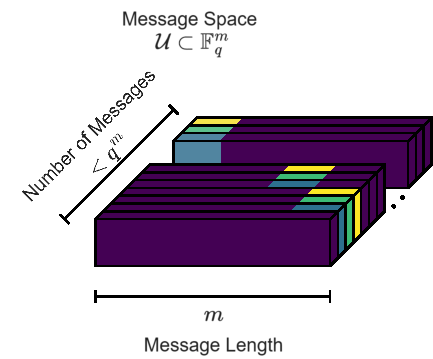
\includegraphics[height=6cm, keepaspectratio]{Poster/figures/ID_flow-Message Patterns.pdf} % Standardized options
    \includesvg[height=6cm]{figures/ID_flow-Message Patterns.drawio.svg}
    \par}
    
    \vfill % This pushes the following text to the bottom of the column
    
    Not in any case, the whole message space is used. The encoding process should be able to convert a narrow message distribution to a uniform tag distribution since this is beneficial with regard to system reliability. Reed-Solomon encoding performs very well whereas Reed-Muller does not achieve this objective.
    
    \columnbreak
    
    % --- COLUMN 2: k-Identification ---
    \subsubsection*{k-Identification}
    {\centering
    %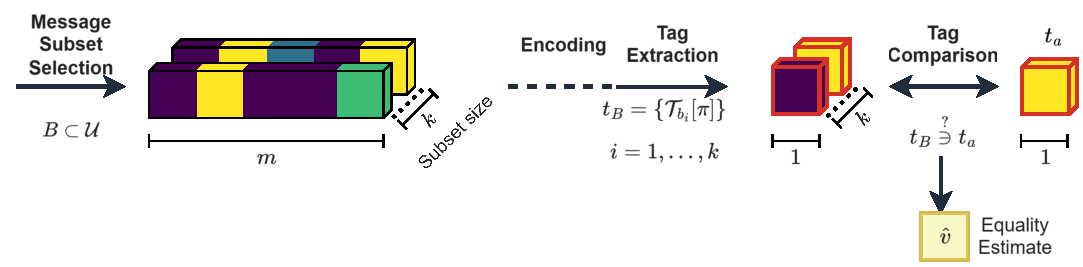
\includegraphics[width=\linewidth, keepaspectratio]{Poster/figures/ID_flow-k-ID.drawio.pdf}
    \includesvg[width=\linewidth]{figures/ID_flow-k-ID.drawio.svg}
    \par}

    %\vfill % This pushes the following text to the bottom of the column

    In k-Identification, the receiver groups messages into subsets and tries to determine whether the received tag matches to at least one of the tags in this subset. This gives the system more tolerance, which is expressed in an increased success probability $ \mathbb{P}(\boldsymbol{a} \in B)$. However, error probability is increased if the right message is not in the subset. Thus, an appropriate partitioning of messages into subsets is crucial.
    
    \columnbreak
    
    % --- COLUMN 3: Multiple Tag Transmission ---
    \subsubsection*{Multiple Tag Transmission}
    {\centering
    %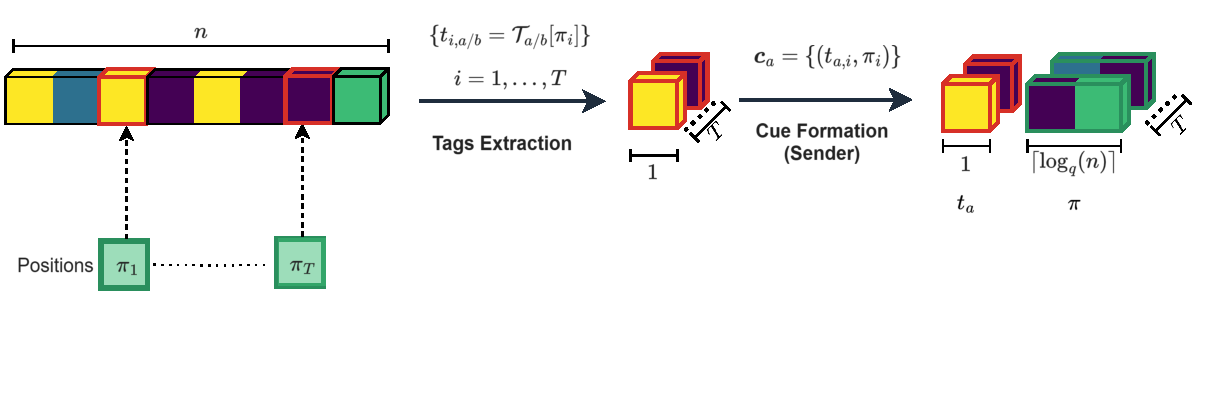
\includegraphics[width=\linewidth, keepaspectratio]{Poster/figures/ID_flow-Multitag.drawio.pdf}
    \includesvg[width=\linewidth]{figures/ID_flow-Multitag.drawio.svg}
    \par}

    An approach to improve system reliability is the transmission of multiple tags. This exponentially decreases error probability while also decreasing code rate. To address this problem, we propose a protocol of subsequent tag transmission. A follow-up tag is only transmitted if the previous all yielded a positive equality estimate, reducing the average number of tags at the cost of a feedback channel and additional processing.
\end{multicols}

\end{document}